\setchapterimage{fig_00}
\chapter*{TD \arabic{cptTD} \\ 
Tête de découpe de tissus -- \ifprof Corrigé \else Sujet \fi}

\addcontentsline{toc}{section}{TD \arabic{cptTD} : Tête de découpe de tissus -- \ifprof Corrigé \else Sujet \fi}

\iflivret \stepcounter{cptTD} \else
\ifprof  \stepcounter{cptTD} \else \fi
\fi
\setcounter{question}{0}

\marginnote{Concours CCINP MP 2018.}
\marginnote{\UPSTIcompetence[2]{B2-07}}
\begin{marginfigure}
\centering
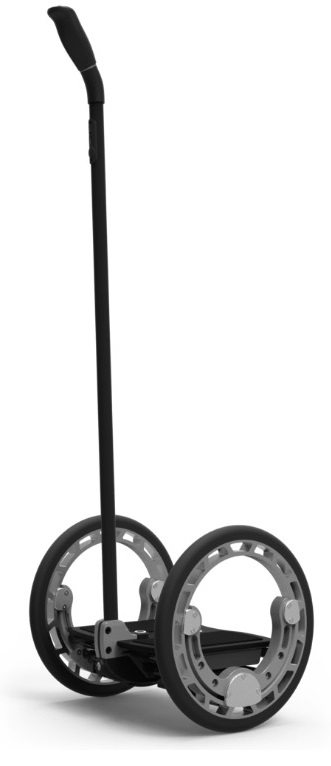
\includegraphics[width=.9\linewidth]{fig_01}
\end{marginfigure}


Un système de découpe automatisé de tissus est composé (figure \ref{fig_02}):
\begin{itemize}
\item d’une table de découpe sur laquelle le tissus à découper (appelé matelas) est maintenu en position
par aspiration;
\item d’un bras transversal qui se déplace en translation de direction $\vect{y_0}$ par rapport à la table;
\item d’une tête de coupe qui se déplace en translation de direction $\vect{x_0}$ par rapport au bras transversal;
\item d’un ordinateur qui pilote l’ensemble du système.
\end{itemize}


\begin{figure}[!h]
\centering
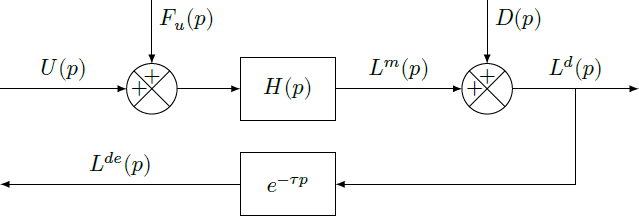
\includegraphics[width=8cm]{fig_02}
\caption{Structure d’une table de découpe de tissus}
\label{fig_02}
\end{figure}

\begin{marginfigure}
\centering
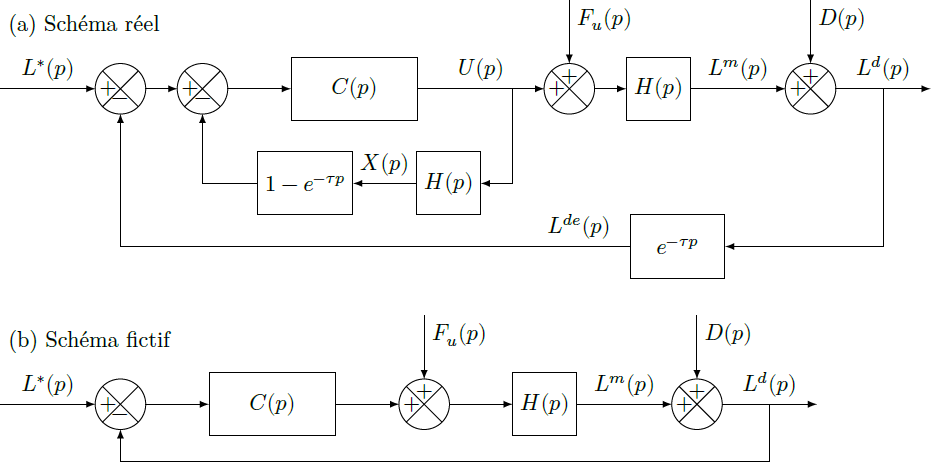
\includegraphics[width=\linewidth]{fig_04}
\caption{Exigence 1.2.2.1}
\label{fig_04}
\end{marginfigure}


\subsection*{Modélisation du comportement du moteur de coupe}
\begin{obj} 
Modémliser la chaîne d’asservissement en vitesse du moteur afin de déterminer les paramètres du correcteur permettant de respecter l’exigence 1.2.2.1 (figure \ref{fig_04}).
\end{obj}

Le mouvement de coupe est asservi en vitesse. La vitesse de rotation du moteur, notée $\omega_m(t)$, est
le paramètre asservi. Elle est mesurée à l’aide d’un codeur incrémental et de son conditionneur qui
fournissent une tension $\indice{u}{mes}(t)$, image de la vitesse de rotation du moteur. Cette tension est comparée à
la tension consigne $\indice{u}{cons}(t)$, image de la vitesse de rotation de consigne $\indice{\omega}{cons}(t)$; un adaptateur fournit $\indice{u}{cons}(t)$ à partir de $\indice{\omega}{cons}(t)$. La tension écart $\varepsilon(t) = \indice{u}{cons}(t) - \indice{u}{mes}(t)$ est alors transformée en tension
d’alimentation du moteur $\indice{u}{m}(t)$ par l’ensemble correcteur-variateur.


\begin{question}
Compléter le schéma-bloc fonctionnel en indiquant dans les blocs
le nom des composants (moteur, adaptateur, correcteur-variateur, capteur-conditionneur) et les
paramètres qui transitent entre les blocs.
\end{question}
\ifprof
\begin{corrige}
\footnotesize
%\begin{figure}[!h]
\begin{center}
\begin{tikzpicture}
\sbEntree{E}

\sbBloc[5]{b0}{Adapt.}{E}
    \sbRelier[$\omega_{\text{cons}}(t)$]{E}{b0}

\sbComp{c1}{b0}
    \sbRelier{b0}{c1}

\sbBloc[3]{b1}{Correct. -- variateur}{c1}
    \sbRelier[$\varepsilon(t)$]{c1}{b1}
    
\sbBloc[3]{b2}{Moteur}{b1}
    \sbRelier[$u_m(t)$]{b1}{b2}
    

\sbSortie[4]{S}{b2}
    \sbRelier{b2}{S}
    \sbNomLien[0.8]{S}{$\omega_m(t)$}
  
%\sbRenvoi{b2-S}{c1}{}


%% BLOC DE RETOUR ET RENVOI
\sbDecaleNoeudy[4]{b2}{n1} 
\sbDecaleNoeudx[0]{n1}{n2} 

\sbBlocr{r}{Capteur}{n2} 
\sbRelieryx{b2-S}{r}
\sbRelierxy[$\indice{u}{mes}(t)$]{r}{c1}
%%%%

\end{tikzpicture}
\end{center}


\normalsize
%%%%%%%%%%%%%%%
\end{corrige}
\else
%%%%%%%%%%%%%%%%%%%%%
\footnotesize
\begin{figure}[!h]
\begin{center}
\begin{tikzpicture}
\sbEntree{E}

\sbBloc[5]{b0}{ }{E}
    \sbRelier[$\omega_{\text{cons}}(t)$]{E}{b0}

\sbComp{c1}{b0}
    \sbRelier{b0}{c1}

\sbBloc[3]{b1}{}{c1}
    \sbRelier{c1}{b1}
    
\sbBloc[3]{b2}{ }{b1}
    \sbRelier[$ $]{b1}{b2}
    

\sbSortie[4]{S}{b2}
    \sbRelier{b2}{S}
    \sbNomLien[0.8]{S}{$\omega_m(t)$}
  
%\sbRenvoi{b2-S}{c1}{}


%% BLOC DE RETOUR ET RENVOI
\sbDecaleNoeudy[4]{b2}{n1} 
\sbDecaleNoeudx[0]{n1}{n2} 

\sbBlocr{r}{}{n2} 
\sbRelieryx{b2-S}{r}
\sbRelierxy{r}{c1}
%%%%

\end{tikzpicture}
\end{center}

\end{figure}
\normalsize
%%%%%%%%%%%%%%%
\fi



On donne les quatre équations du modèle d’un moteur à courant continu :
$u_m(t) = Ri(t) + L \dfrac{\dd i(t)}{\dd t} + e(t)$, 
$J \dfrac{\dd \omega_m(t)}{\dd t} = c_m(t) + c_r(t)$, 
$c_m(t) = k_c i(t)$, $e(t) = k_e\omega_m(t)$.
La fonction de transfert du moteur est notée $H_m(p)=\dfrac{\Omega_m(p)}{U_m(p)}$.

\marginnote{
Le moteur utilisé est un moteur à courant continu dont les caractéristiques et les grandeurs physique sont sont :
\begin{itemize}
\item $R$, résistance de l’induit;
\item $L$, inductance de l’induit;
\item $k_e$, constante de vitesse;
\item $k_c$, constante de couple;
\item $u_m(t)$ est la tension d’alimentation du moteur;
\item $i(t)$ est l’intensité traversant l’induit;
\item $e(t)$ est la force contre-électromotrice;
\item $\omega_m(t)$ est la vitesse de rotation de l’arbre moteur;
\item $c_m(t)$ est le couple moteur;
\item $c_r(t)$ est le couple résistant;
\item $J$ est le moment d’inertie de l’ensemble en mouvement ramené à l’arbre moteur, supposé
constant dans cette partie.
\end{itemize}}

\begin{question}
Transformer les quatre équations dans le domaine de Laplace en supposant les conditions
initiales nulles.
\end{question}
\ifprof
\begin{corrige}
On a $U_m(p) = RI(p) + L pI(p) + E(p)$, 
$J p\Omega_m(p) = C_m(p) + C_r(p)$, 
$C_m(p) = k_c I(p)$, 
$E(p) = k_e\Omega_m(p)$.
\end{corrige}
\else
\fi




\begin{question}
En supposant le couple résistant nul, $c_r(t) = 0$, donner la forme canonique de la fonction de
transfert $H_m(p)$ en fonction de $R$, $L$, $k_e$, $k_c$ et $J$.
\end{question}
\ifprof
\begin{corrige}
On a $U_m(p) = RI(p) + L pI(p) + E(p)$
$ =  \dfrac{C_m(p)}{k_c} \left(R+ Lp\right) + k_e\Omega_m(p) $
$J p\Omega_m(p) = C_m(p) + C_r(p)$, 


\end{corrige}
\else
\fi


\subsection*{Optimisation des performances de l’asservissement en vitesse du moteur}
\begin{obj}
Analyser les performances de l’asservissement en vitesse du moteur afin de concevoir un
correcteur permettant de vérifier l’exigence 1.2.2.1.
\end{obj}

Le correcteur de l’asservissement en vitesse du moteur est un proportionnel-intégrateur de fonction
de transfert $\indice{H}{cor}(p) = K_p+\dfrac{K_i}{p}$.

Les résultats de simulation de la réponse du moteur $\indice{N}{m}(t)$, en boucle fermée, pour une entrée échelon
d’amplitude $N_0 = \SI{3 000}{tr.min^{-1}}$ pour différentes valeurs de $K_p$ et de $K_i$ sont donnés sur la figure \ref{fig_05}.


\begin{marginfigure}
\centering
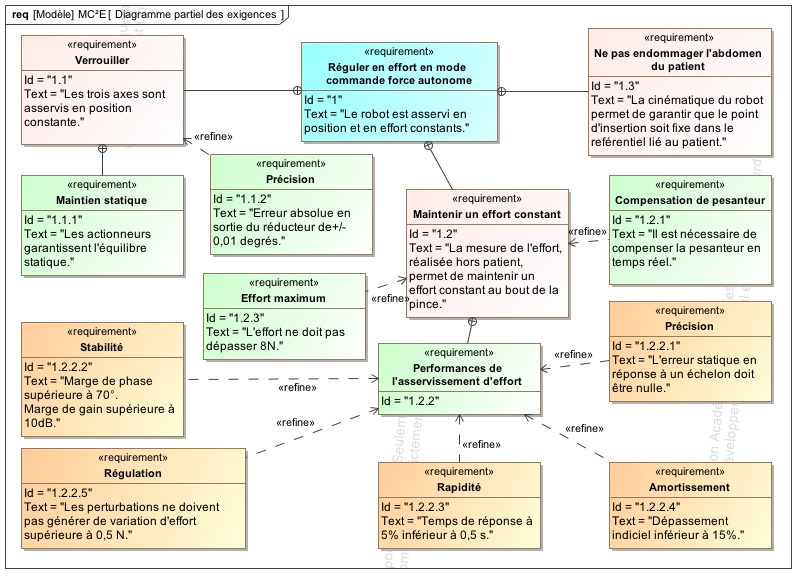
\includegraphics[width=\linewidth]{fig_05}
\caption{Évolutions simulées de $\omega_m(t)$.}
\label{fig_05}
\end{marginfigure}

\begin{question}
Pour chaque courbe de la figure \ref{fig_05}, préciser, en le justifiant, si la valeur de Ki est nulle ou non.
\end{question}
\ifprof
\begin{corrige}
\end{corrige}
\else
\fi


\begin{question}
Pour les courbes 1 et 2, préciser, en le justifiant, la simulation qui est associée à la plus grande
valeur de $K_p$.
\end{question}
\ifprof
\begin{corrige}
\end{corrige}
\else
\fi


\begin{question}
Déterminer les valeurs associées aux quatre critères de performances de l’exigence 1.2.2.1.
Conclure sur le correcteur à adopter.
\end{question}
\ifprof
\begin{corrige}
\end{corrige}
\else
\fi


\ifcolle
\else
\ifprof
\else
\marginnote{
\begin{solution}
\begin{enumerate}[wide, labelwidth=!, labelindent=0pt]
\item Asservissement en position.
\item $H_{\Omega}(p)= \dfrac{K_2}{Jp+K_2}$.%{1}/\left(\dfrac{Jp}{C_{\Omega} K_2}+1 \right) $.
\item $\varepsilon(p)=\dfrac{ \theta_{mC}(p)}{1+H_{\Omega}(p) \dfrac{K_1}{p}}$
\item $\varepsilon(p)= 0, \varepsilon_v = \dfrac{1}{K_1}$   et $K_1 >100$.
\item $\varepsilon_a = \infty$.
\item $\varepsilon(p) = \theta_{mC}(p)\dfrac{p\left( 1+Tp-K_3\right) }{p \left( 1+Tp\right)+K_1} $.
\item $\varepsilon_v =\dfrac{1-K_3}{K_1}$, $K_3=1$.
\item $\varepsilon_a = \dfrac{33\times 10^{-3}}{100} $. Le cahier des charges est donc validé. 
\end{enumerate}
\end{solution}}
\fi
\fi


